\documentclass[tikz]{standalone}
\usepackage{amsmath}
\usetikzlibrary{matrix}
%% EXTRA_TIKZ_PREAMBLE_CODE %%
\begin{document}
%% TIKZ_CODE %%

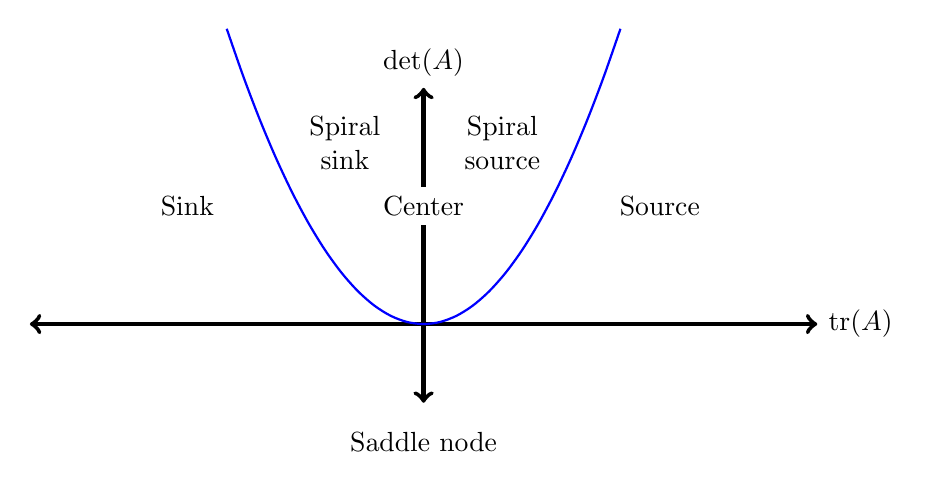
\begin{tikzpicture}
%\draw[help lines, color=gray!30, dashed] (-4.9,-4.9) grid (4.9,4.9);
\draw[<->,ultra thick] (-5,0)--(5,0) node[right]{tr$(A)$};
\draw[<->,ultra thick] (0,-1)--(0,3) node[above]{det$(A)$};
\draw[thick,scale=0.5,domain=-5:5,smooth,variable=\x,blue] plot ({\x},{0.3*\x*\x});
\node at (0,-1.5) {Saddle node};
\node at (-3,1.5) {Sink};
\node at (3,1.5) {Source};
\node[fill=white] at (0,1.5) {Center};
\node[align=center] at (1,2.3) {Spiral \\ source};
\node[align=center] at (-1,2.3) {Spiral \\ sink};
\end{tikzpicture}

\end{document}
